\section{Training Algorithm}
\label{sec:trainer}

\begin{figure}[!ht]
  \centering  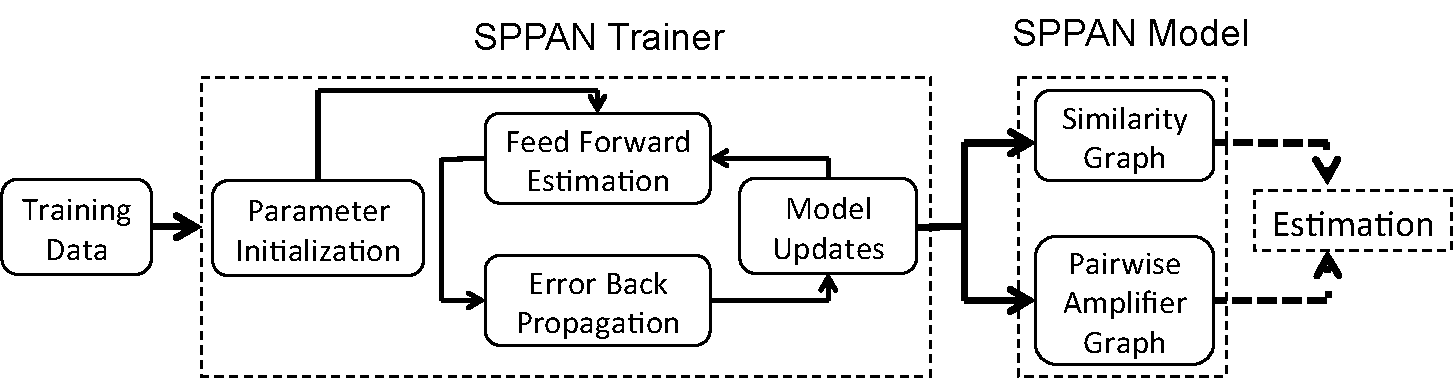
\includegraphics[width=0.5\textwidth]{figures/model.pdf}
  \caption{SPAN system overview.}
  \label{fig:model}
\end{figure}

The mainl workflow of SPAN model is summarized in
Figure~\ref{fig:model}.  The training dataset can be regarded as a
sparse 2D matrix with known entries shown in Figure
\ref{fig:problem-as-matrix}.  Given the training dataset, the training
process starts with a set of initial parameters, then there is an
update loop between feeding forward estimation and backword
propogation, in which {\it Feed Forward Estimation} uses the given
data points to estimate the value of a target entry.  {\it Error Back
  Propagation} updates current model parameters.  The training process
is in an incrementally update way, and generate the final model which
is composed of similarity graph and pairwise amplifier graph. The
learned SPAN model will be directly used to estimate missing values.
In the following sections, we will discuss each component in details.

%The "SPPAN Trainer" is the training module of our proposed SPPAN
%model, which will be further discussed in
%Section~\ref{sec:trainer}. % The output of "SPPAN Trainer" is the
%trained SPPAN model which consists of two major components in SPPAN
%model:(1) Similarity Graph, and (2) Pairwise Amplifier Graph. We will
%cover both components in Section \ref{sec:simi_graph} and
%\ref{sec:pag}.  Consider the advertisement traffic estimation problem
%described in Section~\ref{sec:intro}, The trained SPPAN model will be
%used to estimate the values of interested missing entries in that
%matrix.

\subsection{Feed Forward Estimation}
\label{sec:ffe}

\begin{figure}[!ht]
  \centering
  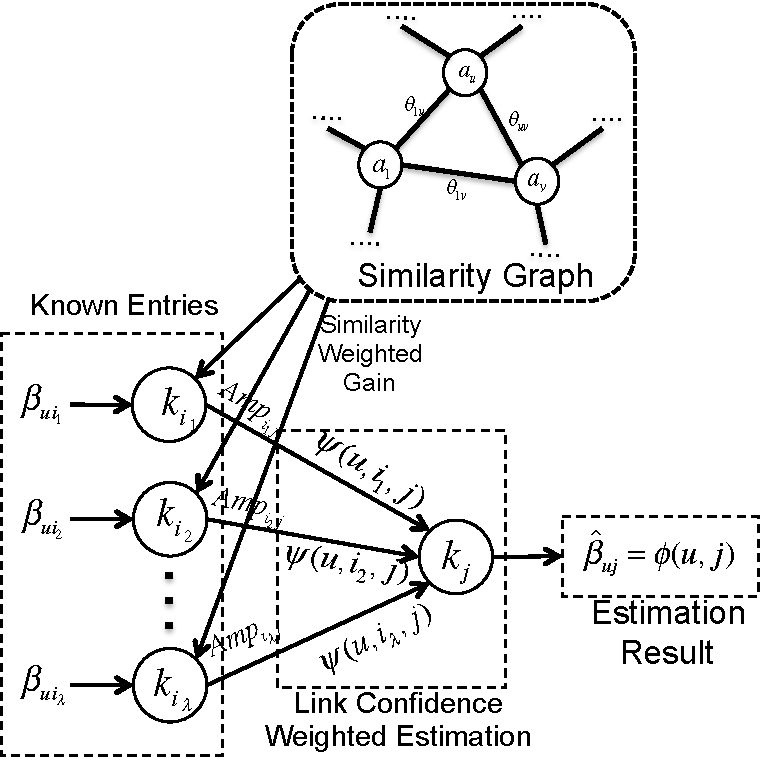
\includegraphics[width=0.43\textwidth]{figures/trainer_feedforward.pdf}
  \caption{Feed Forward Estimation}
  \label{fig:trainer-feedforward}
\end{figure}

\textcolor{red}{ADD MORE DESCRIPTION HERE, need to understand what is
  two layers calculation units? ...}

Given particular values for initial parameters and the inputs data, to
predict parameter settings that minimize the error, our model uses
feed-forward network: the inputs feed into a layer of hidden units,
which can feed into layers of more hidden units, which eventually feed
into the output layer. Each of the hidden units is a squashed linear
function of its inputs.

Our SPAN model uses known entry values $\{\beta_{ui_1}, \beta_{ui_2},
\cdots, \beta_{ui_\lambda}\}$ (where $\lambda$ is the number of known
entry values of advertiser $u$) to estimate the value of target entry
$\beta_{uj}$.  It uses feed forward network to estimate the parameters
in a layer-by-layer way: takes known entry values as inputs, it goes
through a two layers of calculation units to get the final estimated
result.  Similarity weighted sum of entry estimation (in Equation
\ref{eq:feedforward_1}.) and a link confidence weighted sum of entry
estimation (in Equation \ref{eq:feedforward_2} ) are used to estimate
the value of an unknown entry $\beta_{uj} \in \Lambda$ .

As shown in Figure \ref{fig:trainer-feedforward}, the first layer make
estimation of target $\beta_{uj}$ using $\{\beta_{ui_1}, \beta_{ui_2},
\cdots, \beta_{ui_\lambda}\}$ separately with equation
\ref{eq:feedforward_2}, which generates $\lambda$ output estimated
values. The second layer takes all the output estimations from the
first layer $\{\psi(u,i_1,j),\psi(u,i_2,j),\cdots
\psi(u,i_\lambda,j)\}$ as inputs to calculate the final prediction
using equation \ref{eq:feedforward_1}.

\newcommand{\wconf}[3]{\sum\limits_{{#2}:\beta_{{#1}{#2}}\in\Gamma_{({#1},*)}} \confi{{#2}{#3}}\cdot \psi({#1},{#2},{#3})}
\newcommand{\sconf}[3]{\sum\limits_{{#2}:\beta_{{#1}{#2}}\in\Gamma_{({#1},*)}} \confi{{#2}{#3}}}

\newcommand{\wtheta}[2]{\sum \limits_{{#2}:(a_{#2},\gain{{#2}}{ij})\in\amp{ij}} \theta_{{#1}{#2}} \cdot \gain{{#2}}{ij}}
\newcommand{\stheta}[2]{\sum \limits_{{#2}:(a_{#2},\gain{{#2}}{ij})\in\amp{ij}} \theta_{{#1}{#2}}}

\begin{equation}
  \label{eq:feedforward_2}
  \begin{cases}   
    \psi (u,i,j) = \frac{\sum \limits_{v\in V} \theta_{uv} \cdot \gain{{v}}{ij}}{\sum \limits_{v\in V} \theta_{uv}} \cdot \beta_{ui} \\
    V=\{v|(a_{v},\gain{{v}}{ij})\in\amp{ij}\}
   \end{cases}
\end{equation}

\begin{equation}
  \label{eq:feedforward_1}
  \begin{cases}    \hat{\beta}_{uj}=\phi(u,j)=\frac{\sum\limits_{i\in I} \confi{ij}\cdot \psi(u,i,j)}{\sum\limits_{i\in I} \confi{ij}} \\
  	    I=\{i|\beta_{ui}\in\Gamma_{(u,*)}\}
  \end{cases}
\end{equation}

\subsection{Error Back Propagation}
\label{sec:bp}

In Feed Forward Estimation process , we assume the similarity
parameters of advertiser pairs ( in Similarity Graph) and the link
confidence parameters in the Pairwise Amplifier Graph are
given. Indeed the model needs to learn these parameters from the
training dataset using error back proprgation.  The idea of error back
propagation is very similar to artificial neural networks: for an
entry in the training dataset, we hide this entry from the rest of the
training dataset and use the feed forward estimation algorithm in
Section~\ref{sec:ffe} to estimate its value with the rest of the
training dataset. Then we compare the true value of that entry with
current estimation, and back propagate the estimation error (the
deviation from estimated value to the true value) to update the
parameters.  The idea is shown in
Figure~\ref{fig:trainer-train-entry}.  Gradient descent method
\cite{?} is used to optimize the model parameters, which calculates
the gradient of a loss function with respects to all the weights in
the network. The gradient is fed to the optimization method which in
turn uses it to update the weights, in an attempt to minimize the loss
function.

Before developing the parameter update function, we need to calculate
the derivative of the squared error function with respect to all the
parameters in SPAN model, including both
$\{\theta_{uv}\}_{u,v\in[1,N_a]}$ and
$\{\confi{ij}\}_{(i,j):(k_i,k_j)\in E(G_{amp})}$.

The objective function of the parameter optimization problem is shown
in Equation \ref{eq:sum-square-err}, which is the sum of squared
estimation error for all the entries in the training dataset.

\begin{figure}[!ht]
  \centering
  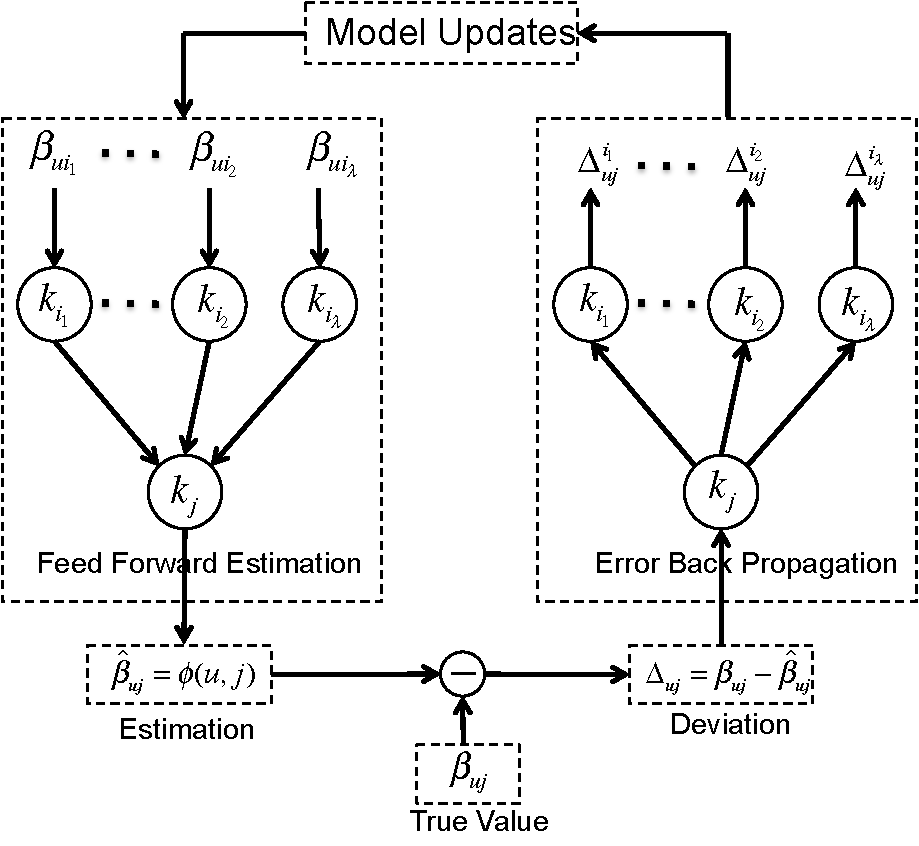
\includegraphics[width=0.49\textwidth]{figures/trainer_train_entry.pdf}
  \caption{The Loop of the Parameter Update}
  \label{fig:trainer-train-entry}
\end{figure}

\begin{equation}
  \label{eq:sum-square-err}
  \begin{aligned}
    J &= \frac{1}{2} \sum_{u,i:\beta_{ui}\in\Gamma} \left(\beta_{ui}-\hat{\beta}_{ui}\right)^2 \\
    &= \frac{1}{2} \sum_{u,i:\beta_{ui}\in\Gamma} \left(\beta_{ui}-\phi(u,i)\right)^2 \\
    &= \frac{1}{2} \sum_{u,i:\beta_{ui}\in\Gamma} \Delta^2_{ui}
  \end{aligned}
\end{equation}

Where $\beta_{ui}$ is the true value, and $\hat{\beta}_{ui}=\phi(u,i)$
is the estimated value given by Feed Forward Estimation algorithm we
described in Section~\ref{sec:ffe}. The factor of $\frac{1}{2}$ at the
beginning of the objective function is a constant factor which would
simplify the expression after the differentiation operation. Noted
that an arbitrary learning rate factor will be multiplied with this
expression in our later learning process, so that it doesn't make any
differences if a constant coefficient is introduced here.

With Equation \ref{eq:feedforward_2}, \ref{eq:feedforward_1} and
\ref{eq:sum-square-err}, the derivatives of our objective function
with respect to parameters $\{\theta_{uv}\}_{u,v\in[1,N_a]}$ and
$\{\confi{ij}\}_{i,j\in[1,N_k]}$ are
\[
\pa{J}{\theta_{uv}} = \sum_{j:\beta_{uj},\beta_{vj}\in\Gamma} \pa{\left[\frac{1}{2}\left(\beta_{uj}-\hat{\beta}_{uj}\right)^2\right]}{\theta_{uv}}
\]
and
\[
\pa{J}{\confi{ij}} = \sum_{u:(a_u,\gain{u}{ij})\in\amp{ij}} \pa{\left[\frac{1}{2}\left(\beta_{uj}-\hat{\beta}_{uj}\right)^2\right]} {\confi{ij}}
\]

With further formula deductions, we can have Equation
\ref{eq:simi_dev} as the derivative result of the objective function
with respect to $\{\theta_{uv}\}_{u,v\in[1,N_a]}$, and Equation
\ref{eq:conf_dev} as the derivative result of the objective function
with respect to $\{\confi{ij}\}_{i,j\in[1,N_k]}$.

\begin{equation}
  \label{eq:simi_dev}
  \begin{cases}
    \pa{J}{\theta_{uv}}=\sum\limits_{j\in J} \sum\limits_{i\in I} \frac{-\Delta_{uj}^{i}}{\sum \limits_{v'\in V} \theta_{{u}{v'}}}  \left(\gain{v}{ij}\cdot\beta_{ui}- \psi(u,i,j)\right) \\
    J=\{j|\beta_{uj},\beta_{vj}\in\Gamma\} \\
    I=\{i|\beta_{ui}\in\Gamma_{(u,*)}\} \\
    V=\{v|(a_{v},\gain{{v}}{ij})\in \amp{ij}\}
  \end{cases}
\end{equation}

\begin{equation}
  \label{eq:conf_dev}
  \begin{cases}
    \pa{J}{\confi{ij}}=\sum\limits_{u\in U} \left[ -\frac{\Delta_{uj}}{\sum\limits_{i'\in I} \confi{{i'}{j}}} \left(\psi(u,i,j) - \phi(u,j)\right) \right] \\
    U=\{u|(a_u,\gain{u}{ij})\in\amp{ij}\} \\
    I=\{i:\beta_{{u}{i}}\in\Gamma_{({u},*)}\}
  \end{cases}
\end{equation}

where $\Delta_{uj}$ is the estimation error and $\Delta_{uj}^{i}$ is
back propagated error, their expressions are given by
Equation~\ref{eq:derivative_condition}.

\begin{equation}
  \label{eq:derivative_condition}
  \begin{cases}
    \Delta_{uj}=\beta_{uj}-\hat{\beta}_{uj}\\
    \Delta_{uj}^{i}=\frac{\confi{ij}}{\sconf{u}{i'}{j}}\cdot \Delta_{uj}
  \end{cases}
\end{equation}

With the derivatives and back propagated errors given by Equation
\ref{eq:simi_dev}, \ref{eq:conf_dev} and
\ref{eq:derivative_condition}, we can update the parameter of SPPAN
model in the Similarity Graph and the Pairwise Amplifier Graph using
the gradient descent approach. Given a specific learning rate $\eta$,
the changes of model parameters are equal to the product of the
learning rate and the corresponding gradient value, multiplied by
-1. Therefore, the parameter update function for training target
$\beta_{uj}$ can be expressed in Equation \ref{eq:gradient descent}.

\begin{equation}
  \label{eq:gradient descent}
  \begin{cases}
    \confi{ij} := \confi{ij}-\eta \cdot \pa{J}{\confi{ij}}\\
    \theta_{uv} := \theta_{uv} -\eta \cdot \pa{J}{\theta_{uv}}
  \end{cases}
\end{equation}

\noindent where $\pa{J}{\confi{ij}}$ and $\pa{J}{\theta_{uv}}$ are
given by Equation \ref{eq:simi_dev}, \ref{eq:conf_dev} and
\ref{eq:derivative_condition}. Figure \ref{fig:trainer-train-entry}
shows the parameter update loop of the Feed Forward Estimation and the
Error Back Propagation for a training target entry $\beta_{uj}$.

\subsection{Training Algorithm for SPAN model}
Combining the Feed Forward Estimation and Error Back Propagation, The
training algorithm for SPPAN model can be summarized in Algorithm
\ref{alg:training}.

The stop criterion for the training algorithm is a training error
threshold: the training will stop if the training error drops to a
specific value. Other criterion may also be used, such as maximum
iteration number\cite{?}, error reduction rate threshold\cite{?}, the
convergence of the parameters\cite{?} and so on.

The training algorithm generates final SPAN model, which includes the
Similarity Graph and Pairwise Amplifier Graph. To estimate unknown
entries, we can just follow the Feed Forward Estimation described in
Section \ref{sec:ffe}, using the well-trained Similarity Graph and
Pairwise Amplifier Graph.


\begin{algorithm}
  \KwData{The set of given/known entries $\Gamma$ in matrix $M$\\
    ~~~~~~~~~Learning rate $\eta$\\
  }
  \KwResult{$\{\theta_{uv}\}_{u,v\in[1,N_a]}$ in adgroups similarity graph \\
    ~~~~~~~~~~~~$\{\confi{ij}\}_{(i,j):(k_i,k_j)\in E(G_{amp})}$ in criteria pairwise amplifier graph
  }
  \textbf{Initialization:}\\
  \begin{itemize}
  \item initialize the pairwise amplifier set
    $Amp_{ij}=\{(a_u,\gain{u}{ij})~|~u\in
    [1,N_a],\beta_{ui},\beta_{uj}\in \Gamma\} \cup \{(a_0,c_{ij})\}$
    using $\gain{u}{ij}=\beta_{uj}/\beta_{ui}$
  \item initialize parameters $\{\theta_{uv}\}$ in adgroup similarity
    graph using small random numbers when encountered.
  \item initialize parameters $\{\confi{ij}\}$ in criteria pairwise
    amplifier graph using small random numbers when encountered.
  \end{itemize}
  \Begin{
    \While{stop criterion not meet}{
      \For{each $\beta_{uj}$ in $\Gamma$}{
  \tcc{ SPPAN Model feed forward estimation of training example $\beta_{uj}$} 
  \tcc{with Equation~\ref{eq:feedforward_2} and \ref{eq:feedforward_1}}
  $\hat{\beta}_{uj}=FeedForwardEstimation(\mbox{SPPAN Model},u,j)$  \\
  \tcc{error back propagation using Equation~\ref{eq:derivative_condition}}
  $(\Delta_{uj},\{\Delta_{uj}^{i}\})=ErrorBackPropagation(\mbox{SPPAN Model},u,j,\hat{\beta}_{uj})$ \\
  \tcc{update SPPAN model using gradient descent Equation \ref{eq:simi_dev}, \ref{eq:conf_dev} and \ref{eq:derivative_condition}}
  $update(\mbox{SPPAN Model},\Delta_{uj},\{\Delta_{uj}^{i}\})$
      }
    }
    return (\mbox{SPPAN Model})
  }
  \caption{Training Algorithm for SPPAN Model}
  \label{alg:training}
\end{algorithm}

\subsection{Handling Large Scale  Data}
Algorithm \ref{alg:training} works well in most cases. However, as the
data set become much bigger and less sparse, the iterative process of
error back propagation based parameter update for SPPAN model often
take a great deal of time to completely go through the whole training
set.  Another advantage of our model is that it can handle large scale
sparse data in an effective way. As we can see from Algorithm
\ref{alg:training}, the SPPAN model updates can use different
independent training samplesr. Thus, map-reduce techniques can be used
to greatly decrease the amount of time that the training algorithm
takes to converge.

For each training iteration, the mapping part can takes each training
example separately and executes the feed forward and error backward
propagation in parallel to generate model updates. Then, the updates
for all the parameters of SPPAN model are summed up in the reducing
units. At the end of each iteration, the SPPAN model can be updated
using the outputs from the reducing unites. This process continues
until the stop criterion is met.


\subsection{Handling Extreme Sparse Data}

\textcolor{red}{add a section about how to handle extreme sparse data,
  explain why your model can handle extrem sparse data}
